\documentclass[border=0pt]{standalone}
\usepackage{tikz}
\usetikzlibrary{calc}
\definecolor{nighttop}{RGB}{8,12,40}
\definecolor{nightmid}{RGB}{18,28,70}
\definecolor{nighthorizon}{RGB}{45,35,90}
\definecolor{ground}{RGB}{18,14,28}
\definecolor{groundlight}{RGB}{35,28,45}
\definecolor{fireworkred}{RGB}{255,90,70}
\definecolor{fireworkgold}{RGB}{255,210,80}
\definecolor{fireworkcyan}{RGB}{100,220,255}
\definecolor{fireworkpink}{RGB}{255,130,200}
\definecolor{lantern}{RGB}{255,170,50}
\definecolor{lanterncore}{RGB}{255,230,140}
\definecolor{stallwood}{RGB}{55,35,25}
\definecolor{stallroof}{RGB}{140,40,40}
\definecolor{silhouette}{RGB}{12,8,18}
\definecolor{starglow}{RGB}{220,230,255}
\definecolor{waterglow}{RGB}{80,60,120}
\begin{document}
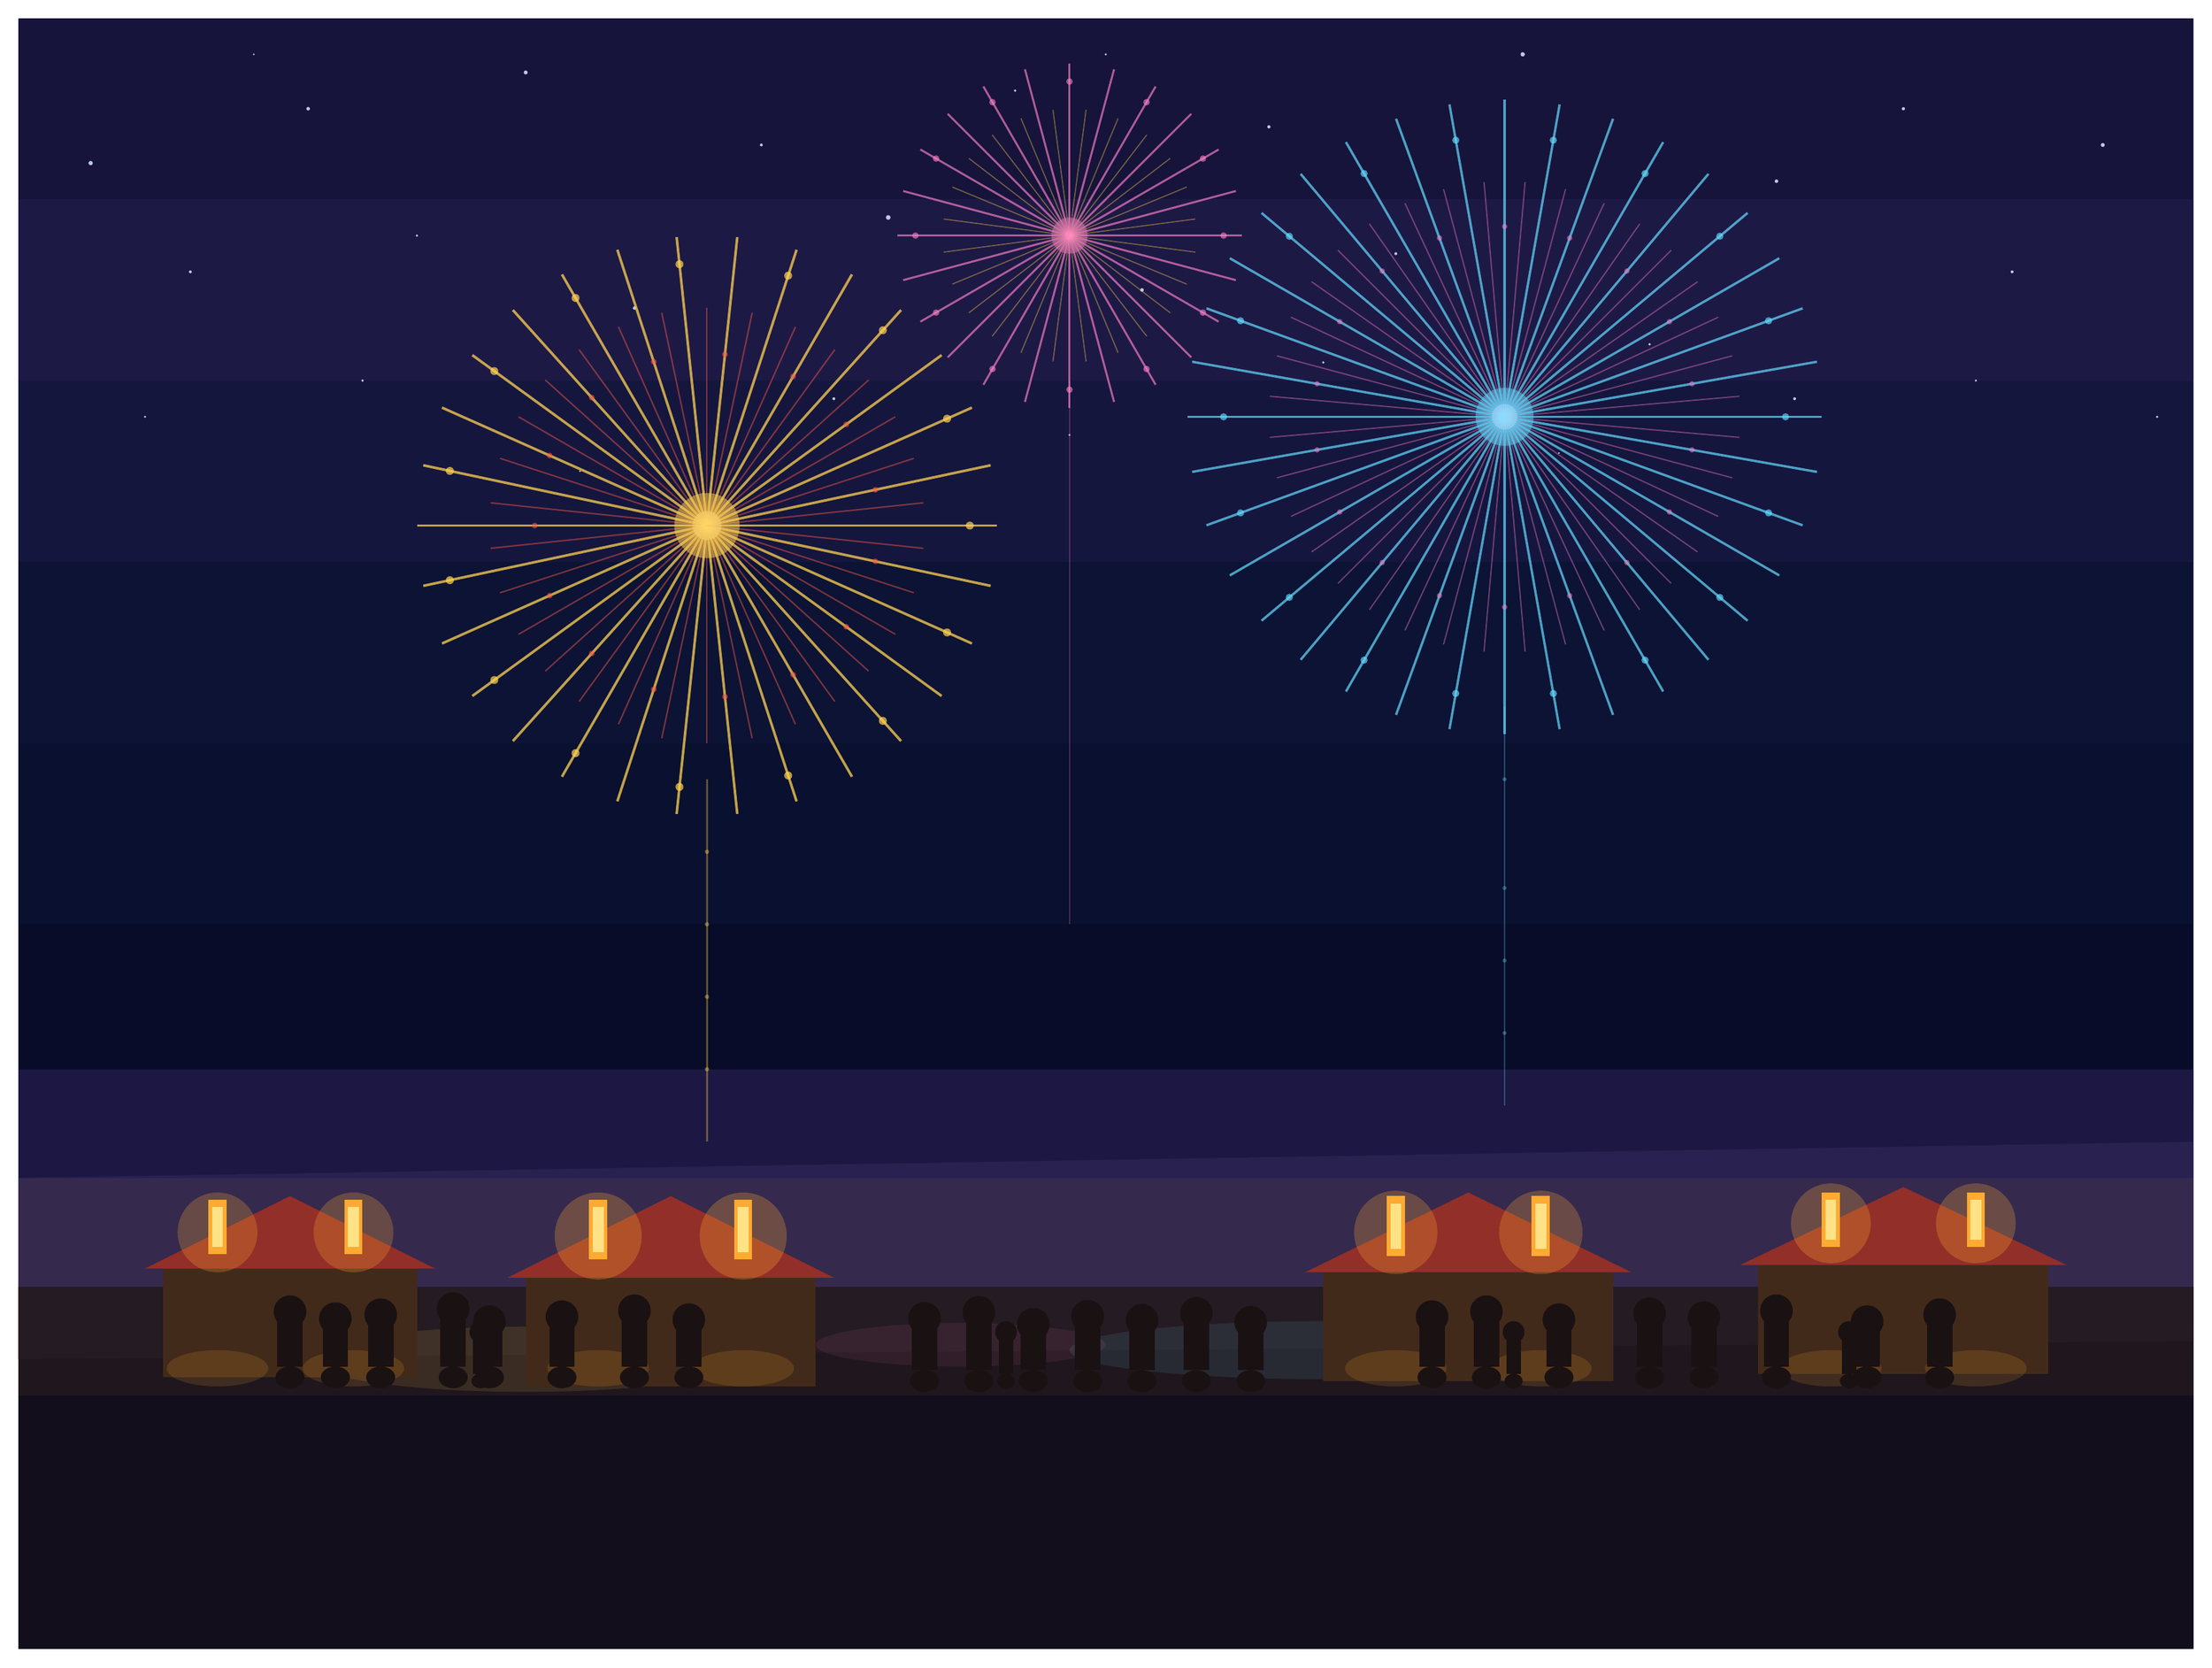
\begin{tikzpicture}[x=1pt,y=1pt]
  % Canvas ~1200x900
  \clip (0,0) rectangle (1200,900);

  % Night sky gradient bands
  \fill[nighttop] (0,0) rectangle (1200,900);
  \foreach \i/\c in {%
    0/nighttop,%
    1/nighttop,%
    2/nightmid,%
    3/nightmid,%
    4/nighthorizon,%
    5/nighthorizon%
  }{%
    \fill[opacity={0.18+\i*0.04},\c] (0,{200+\i*100}) rectangle (1200,{400+\i*100});
  }
  \fill[nighthorizon,opacity=0.55] (0,180) rectangle (1200,320);
  \fill[waterglow,opacity=0.25] (0,160) -- (1200,160) -- (1200,280) -- (0,260) -- cycle;

  % Stars
  \foreach \x/\y/\s in {%
    40/820/1.2, 95/760/0.8, 160/850/1.0, 220/780/0.7, 280/870/1.1,%
    340/740/0.9, 410/830/0.8, 480/790/1.3, 550/860/0.7, 620/750/1.0,%
    690/840/0.9, 760/770/0.8, 830/880/1.2, 900/720/0.7, 970/810/1.0,%
    1040/850/0.9, 1100/760/0.8, 1150/830/1.1, 70/680/0.6, 190/700/0.7,%
    310/650/0.5, 450/690/0.8, 580/670/0.6, 720/710/0.7, 850/660/0.5,%
    980/690/0.8, 1080/700/0.6, 1180/680/0.7, 130/880/0.5, 600/880/0.6%
  }{%
    \fill[starglow,opacity=0.85] (\x,\y) circle (\s);
  }

  % Firework burst helper: center, radius, color, ray count offset
  % Burst 1 — gold/red left-center
  \foreach \a in {0,12,...,348}{%
    \draw[fireworkgold,opacity=0.75,line width=1.4pt]
      (380,620) -- ++({\a}:160);
    \draw[fireworkred,opacity=0.45,line width=0.8pt]
      (380,620) -- ++({\a+6}:120);
  }
  \foreach \a in {0,24,...,336}{%
    \fill[fireworkgold,opacity=0.7] ($(380,620)+({\a}:145)$) circle (2.2);
    \fill[fireworkred,opacity=0.55] ($(380,620)+({\a+12}:95)$) circle (1.6);
  }
  \fill[fireworkgold,opacity=0.5] (380,620) circle (18);
  \fill[lanterncore,opacity=0.35] (380,620) circle (8);

  % Burst 2 — cyan/pink right-center
  \foreach \a in {0,10,...,350}{%
    \draw[fireworkcyan,opacity=0.7,line width=1.3pt]
      (820,680) -- ++({\a}:175);
    \draw[fireworkpink,opacity=0.4,line width=0.7pt]
      (820,680) -- ++({\a+5}:130);
  }
  \foreach \a in {0,20,...,340}{%
    \fill[fireworkcyan,opacity=0.65] ($(820,680)+({\a}:155)$) circle (2.0);
    \fill[fireworkpink,opacity=0.5] ($(820,680)+({\a+10}:105)$) circle (1.5);
  }
  \fill[fireworkcyan,opacity=0.45] (820,680) circle (16);
  \fill[starglow,opacity=0.3] (820,680) circle (7);

  % Burst 3 — pink/gold smaller upper center
  \foreach \a in {0,15,...,345}{%
    \draw[fireworkpink,opacity=0.65,line width=1.1pt]
      (580,780) -- ++({\a}:95);
    \draw[fireworkgold,opacity=0.4,line width=0.6pt]
      (580,780) -- ++({\a+7.5}:70);
  }
  \foreach \a in {0,30,...,330}{%
    \fill[fireworkpink,opacity=0.6] ($(580,780)+({\a}:85)$) circle (1.8);
  }
  \fill[fireworkpink,opacity=0.4] (580,780) circle (10);

  % Rising sparks / trails
  \draw[fireworkgold,opacity=0.35,line width=1.2pt] (380,280) -- (380,480);
  \draw[fireworkcyan,opacity=0.3,line width=1.0pt] (820,300) -- (820,520);
  \draw[fireworkpink,opacity=0.25,line width=0.8pt] (580,400) -- (580,700);
  \foreach \y in {320,360,400,440}{%
    \fill[fireworkgold,opacity=0.4] (380,\y) circle (1.2);
  }
  \foreach \y in {340,380,420,480}{%
    \fill[fireworkcyan,opacity=0.35] (820,\y) circle (1.1);
  }

  % Ground
  \fill[ground] (0,0) rectangle (1200,200);
  \fill[groundlight,opacity=0.4] (0,160) -- (1200,170) -- (1200,200) -- (0,200) -- cycle;

  % Reflections of fireworks on ground
  \fill[fireworkgold,opacity=0.12] (280,160) ellipse (120 and 18);
  \fill[fireworkcyan,opacity=0.10] (720,165) ellipse (140 and 16);
  \fill[fireworkpink,opacity=0.08] (520,168) ellipse (80 and 12);

  % Stalls with lanterns
  % Stall 1
  \fill[stallwood] (80,150) rectangle (220,210);
  \fill[stallroof] (70,210) -- (150,250) -- (230,210) -- cycle;
  \fill[lantern,opacity=0.25] (110,230) circle (22);
  \fill[lantern] (105,218) rectangle (115,248);
  \fill[lanterncore] (107,222) rectangle (113,244);
  \fill[lantern,opacity=0.25] (185,230) circle (22);
  \fill[lantern] (180,218) rectangle (190,248);
  \fill[lanterncore] (182,222) rectangle (188,244);

  % Stall 2
  \fill[stallwood] (280,145) rectangle (440,205);
  \fill[stallroof] (270,205) -- (360,250) -- (450,205) -- cycle;
  \fill[lantern,opacity=0.28] (320,228) circle (24);
  \fill[lantern] (315,215) rectangle (325,248);
  \fill[lanterncore] (317,219) rectangle (323,244);
  \fill[lantern,opacity=0.28] (400,228) circle (24);
  \fill[lantern] (395,215) rectangle (405,248);
  \fill[lanterncore] (397,219) rectangle (403,244);

  % Stall 3
  \fill[stallwood] (720,148) rectangle (880,208);
  \fill[stallroof] (710,208) -- (800,252) -- (890,208) -- cycle;
  \fill[lantern,opacity=0.26] (760,230) circle (23);
  \fill[lantern] (755,217) rectangle (765,250);
  \fill[lanterncore] (757,221) rectangle (763,246);
  \fill[lantern,opacity=0.26] (840,230) circle (23);
  \fill[lantern] (835,217) rectangle (845,250);
  \fill[lanterncore] (837,221) rectangle (843,246);

  % Stall 4
  \fill[stallwood] (960,152) rectangle (1120,212);
  \fill[stallroof] (950,212) -- (1040,255) -- (1130,212) -- cycle;
  \fill[lantern,opacity=0.27] (1000,235) circle (22);
  \fill[lantern] (995,222) rectangle (1005,252);
  \fill[lanterncore] (997,226) rectangle (1003,248);
  \fill[lantern,opacity=0.27] (1080,235) circle (22);
  \fill[lantern] (1075,222) rectangle (1085,252);
  \fill[lanterncore] (1077,226) rectangle (1083,248);

  % Lantern glow on ground
  \foreach \x in {110,185,320,400,760,840,1000,1080}{%
    \fill[lantern,opacity=0.15] (\x,155) ellipse (28 and 10);
  }

  % People silhouettes
  % Group near stall 1-2
  \foreach \x/\h in {150/55,175/48,200/52,240/58,260/45,300/50,340/56,370/47}{%
    \fill[silhouette] (\x,150) ellipse (8 and 6);
    \fill[silhouette] (\x-7,156) rectangle (\x+7,156+\h*0.55);
    \fill[silhouette] (\x,156+\h*0.55) circle (9);
  }
  % Center crowd
  \foreach \x/\h in {500/52,530/58,560/46,590/54,620/50,650/57,680/48}{%
    \fill[silhouette] (\x,148) ellipse (8 and 6);
    \fill[silhouette] (\x-7,154) rectangle (\x+7,154+\h*0.55);
    \fill[silhouette] (\x,154+\h*0.55) circle (9);
  }
  % Right crowd
  \foreach \x/\h in {780/50,810/55,850/47,900/53,930/49,970/56,1020/45,1060/52}{%
    \fill[silhouette] (\x,150) ellipse (8 and 6);
    \fill[silhouette] (\x-7,156) rectangle (\x+7,156+\h*0.55);
    \fill[silhouette] (\x,156+\h*0.55) circle (9);
  }
  % Child silhouettes
  \foreach \x in {255,545,825,1010}{%
    \fill[silhouette] (\x,148) ellipse (5 and 4);
    \fill[silhouette] (\x-4,152) rectangle (\x+4,175);
    \fill[silhouette] (\x,175) circle (6);
  }

  % Soft ambient lantern wash
  \fill[lantern,opacity=0.06] (0,140) rectangle (1200,260);

\end{tikzpicture}
\end{document}
